\subsection{The electron and the nucleus are assumed to possess an angular momentum. What consequences do these angular momenta have?}


Kigger vi først på elektronen, så har denne et baneimpulsmoment ($\Vec{l}$), idet den er i banebevægelse omkring kernen af atomet, og derudover har den også et indre impulsmoment, kaldet spin ($\Vec{s}$), hvilken har størrelsen $s = 1/2$, og dette kan ikke ændres af tilstanden, som elektronen befinder sig i, ligesom baneimpulsmomentet kan. Elektronens spin giver anledning til et dipolmoment
\begin{align}
    \Vec{\mu}_s &= - g_s \frac{\mu_B}{\hbar}\Vec{s} \: ,
\end{align}
hvor $\mu_B = e\hbar/(2m_e)$ er Bohrmagnetronen, og $g_s$ er Landé g-faktoren for elektronens spin\footnote{$g_s \simeq 2$}. Dette dipolmoment vekselvirker med et magnetfelt dannet af elektronens banebevægelse, hvilket kan beskrives ved Hamiltonoperatoren
\begin{align}
    H_{FS} &= - \Vec{\mu}_s \cdot \Vec{B}_l \: ,
\end{align}
hvilket giver anledning til finstrukturenergiskiftet, når vi generaliserer til et vilkårligt antal elektroner, hvorfor $\Vec{J} = \Vec{L} + \Vec{S}$ og $\Vec{L} = \sum_i \Vec{l}_i$ og $\Vec{S} = \sum_i \Vec{s}_i$:
\begin{align}
    E_{FS} &= \frac{\beta}{2} \left\{J(J+1) - L(L+1) - S(S+1)\right\} \: ,
\end{align}
hvor $A \propto \mu_B^2$ er finstrukturkonstanten.

Her har vi betragtet finstruktur ud fra LS-koblingen, men man kunne også betragte denne med jj-koblingen (hvis $E_{re} \gg E_{SO}$ i stedet for $E_{re} \gg E_{SO}$\footnote{Her er $E_{re}$ redsidual electrostatic energy ($\sim \SI{1}{\eV}$) og $E_{SO}$ er energien fra spin-banekoblingen.}), hvor $\Vec{J} = \sum_i j_i$ og $j_i = l_i + s_i$.\\

Betragter vi herudover kernen som havende et impulsmoment ($\Vec{I}$), så giver dette anledning til dipolmomentet
\begin{align}
    \Vec{\mu}_I &= g_I \frac{\mu_N}{\hbar}\Vec{I} \: ,
\end{align}
hvor $\mu_N = e\hbar/(Zm_p)$ er kernemagnetronen, og $g_I$ er Landé g-faktoren for kernens impulsmoment. Dette dipolmoment vekselvirker med det magnetiske felt dannet af elektronerne
\begin{align}
    H_{HFS} &= - \Vec{\mu}_I \cdot \Vec{B}_J \: ,
\end{align}
hvilket giver anledning til hyperfinstrukturenergiskiftet
\begin{align}
    E_{HFS} &= \frac{A}{2} \left\{F(F+1) - I(I+1) - J(J+1)\right\} \: ,
\end{align}
hvor $A \propto \mu_N \mu_B$ er hyperfinstrukturkonstanten.\\

Det kan ses, at disse to energiskifte minder om hinanden -- de er på samme form -- og vi skal også se, at de udledes på meget lignende måder. Det bemærkes også, at både fin- og hyperfinstrukturkonstanten er proportionel med kvadratet på Bohrmagnetronen ($\mu_B^2$), idet
\begin{align}
    \mu_N &= \frac{m_e}{m_p} \mu_B = \frac{1}{1836}\mu_B \simeq \frac{1}{2000}\mu_B \: ,
\end{align}
men som det kan ses, af omregningen fra kernemagnetronen til Bohrmagnetronen, så er der en faktor $\sim 2000$ til forskel, hvorfor finstruktur er af en størrelsesorden $\sim 2000$ større end hyperfinstrukturen. Også heraf kommer navnene ''finstruktur'' og ''hyperfinstruktur'', da man ser hyperfinstrukturen være en perturbation af finstrukturen, som allerede er en perturbation af den fundne energi fra Schrödingerligningen.\\


\paragraph{Overordnet udledning af fin- og hyperfinstruktur (i én):} Både fin- og hyperfinstruktur udeledes fra vekselvirkningen mellem et dipolmoment og et magnetisk felt. Det observeres, at man får en kobling af impulsmomenterne, hvorved man skal skifte basis til hhv. $\ket{L,\: S,\: J,\: M_J}$ for finstrukturen (i jj-koblingen dog basen $\ket{j_1,\: j_2,\: J,\: M_J}$) og $\ket{J,\: I,\: F,\: M_F}$ for hyperfinstrukturen.

Det bliver nødvendigt at beregne forventningsværdien af prikproduktet af de to impulsmomenter, hvis basis, som man skiftede fra, idet $E_{FS} \propto \braket{\Vec{S} \cdot \Vec{L}}$, hvorved man finder
\begin{align}
    \braket{\Vec{S} \cdot \Vec{L}} &= \braket{\frac{\Vec{J}^2 - \Vec{L}^2 - \Vec{S}^2}{2}}
    = \frac{\braket{\Vec{J}^2} - \braket{\Vec{L}^2} - \braket{\Vec{S}^2}}{2} \nonumber\\
    &= \frac{\hbar^2}{2}\left\{J(J+1) - L(L+1) - S(S+1)\right\} \: ,
\end{align}
idet $\Vec{J} = \Vec{L} + \Vec{S}$ for finstruktur, og ligeledes for hyperfinstrukturen: $E_{HFS} \propto \braket{\Vec{J} \cdot \Vec{I}}$, hvor $\Vec{F} = \Vec{I} + \Vec{J} \propto F(F+1) - I(I+1) - J(J+1)$.\\


\paragraph{Eksempel på fin- og hyperfinstrukturopsplitning:} Som eksempel kan vi se på 2P-tilstanden i hydrogen. Her er $n = 2$ og $l = 1$, og siden at vi taler om en enkelt elektron vil $s = 1/2$, hvorfor $j = 1/2,\: 3/2$. Hydrogenkernen består af en enkelt proton, hvilken har spin $1/2$, hvorfor $I = 1/2$. Derved bliver $F = 1,\: 2$ og $F = 0,\: 1$ hhv.. Dette kan ses af \cref{fig:Q16_HyperFineSplittingOf2PstateInHydrogen}.
\begin{figure}[!h]
    \centering
    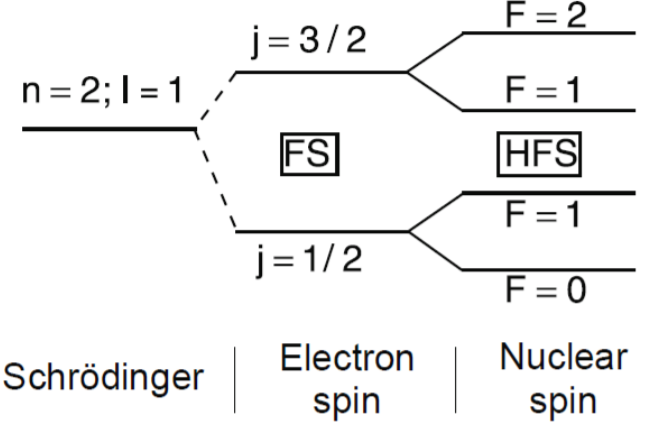
\includegraphics[width=0.70\textwidth]{Q16/images/HyperFineSplittingOf2PstateInHydrogen.PNG}
    \caption{Fin- og hyperfinstrukturopsplitning af 2P-tilstanden i hydrogen. $n = 2$, $l = 1$, så $j = \frac{1}{2}, \: \frac{3}{2}$ og $F = 0,\: 1,\: 2$. Not to scale.}
    \label{fig:Q16_HyperFineSplittingOf2PstateInHydrogen}
\end{figure}